%-----------------------------------------------------------------------------%
\chapter{\babEmpat}
%-----------------------------------------------------------------------------%

%-----------------------------------------------------------------------------%
\section{Petunjuk Penggunaan}
%-----------------------------------------------------------------------------%


%%--------------------------------%
%\todo{
	%\section{Simulasi Sistem}
	%Masukkan gambar simulasi pada gnuradio\\ 
	%Masukkan gambar hasil yang dilakukan dengan simulasi (berupa time vs frequency).\\
	%Masukkan proses analisis yang dilakukan dengan hasil simulasi, seperti langkah konversi biner ke kompleks, penentuan data yang diambil,... pada matlab.\\
	%Lakukan desain blok dari hasil pada matlab menuju python.\\
	%Uji coba blok python yang telah dirancang pada simulasi\\
	%Bandingkan hasilnya dengan pada matlab
	%}
%%--------------------------------%

\begin{figure}
	\centering
	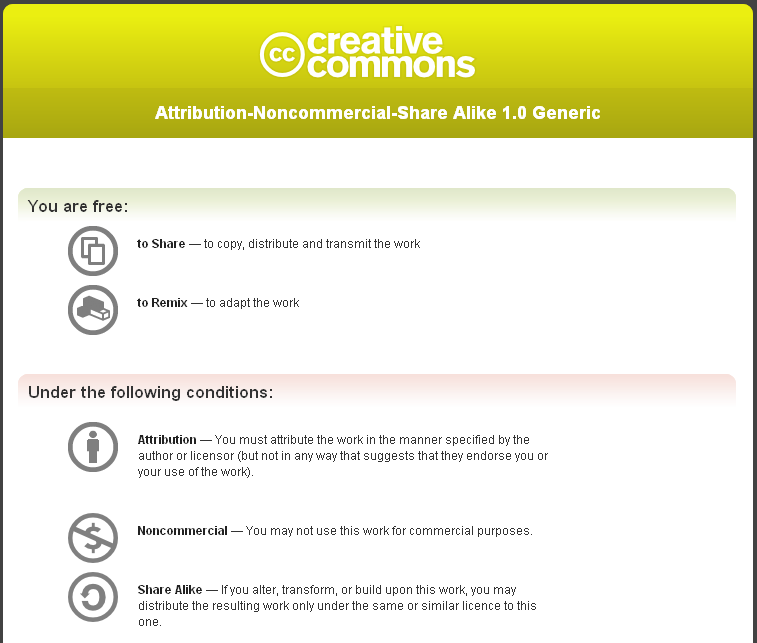
\includegraphics[width=0.3\textwidth]
		{pics/creative_common.png}
		\caption{CC-A-NC-SA 1.0 Generic}
	\label{fig:CC10}
\end{figure}

\textit{Template} tugas ini dipasangkan lisensi \textit{Creative Common---Attribution---Non Commercial---Share Alike 1.0 Generic}.